\section[Case \& Submissions]{\textbf{Case Conditions \& Submission Summary}}

\begin{frame}{\small Geometry and Aerodynamic Conditions}
\scriptsize

\begin{columns}[T,onlytextwidth]

%------------------------------------------------
\begin{column}{0.46\textwidth}
\centering
\begin{figure}
    \centering
    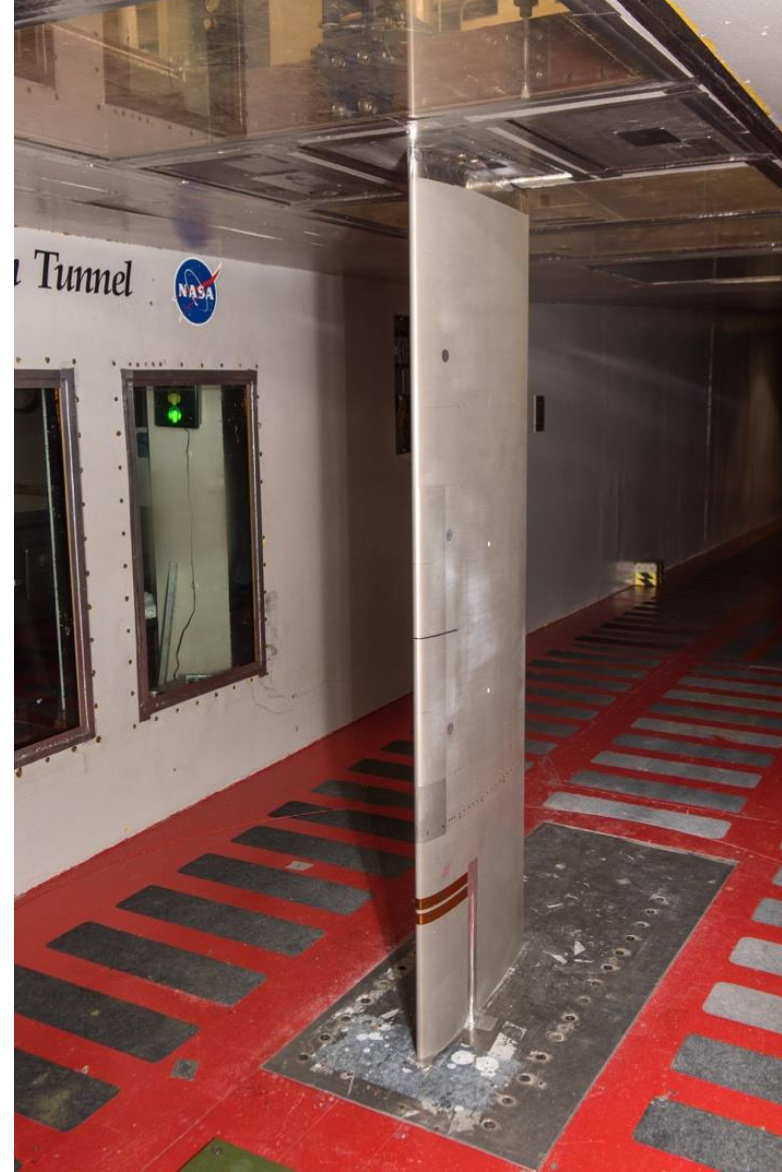
\includegraphics[height=0.66\textheight]{FIGURES_CONDITIONS/NACA0012_TUNNEL_VIEW.png}
\end{figure}

\vspace{-0.15cm}

\centering
\textbf{Wind-Tunnel View}

\end{column}

%------------------------------------------------
\begin{column}{0.50\textwidth}
\centering
\vspace{0.5cm}
\textbf{Geometry}

\vspace{0.15cm}

\begin{tabular}{lc}
\toprule
\textbf{Parameter} & \textbf{Value} \\
\midrule
Airfoil & NACA0012 \\
Chord, $c$ [m] & $0.5334$ \\
AOA, $\alpha$ [$^\circ$] & $4.0$ \\
\bottomrule
\end{tabular}

\vspace{0.35cm}

\textbf{Aerodynamic Conditions}

\vspace{0.15cm}

\begin{tabular}{lc}
\toprule
\textbf{Parameter} & \textbf{Value} \\
\midrule
$T_{0,\mathrm{ref}}$ [K]         & $272.95$ \\
$T_{s,\mathrm{ref}}$ [K]         & $267.75$ \\
$M_{\mathrm{ref}}$ [-]           & $0.3114$ \\
$U_{\mathrm{ref}}$ [m/s]         & $102.15$ \\
$\rho_{\mathrm{ref}}$ [kg/m$^3$] & $1.19$ \\
$Re_{c,\mathrm{ref}}$ [-]        & $3.8441\times10^6$ \\
\bottomrule
\end{tabular}

\end{column}

\end{columns}

\end{frame}

\begin{frame}{\small Icing Conditions}
\scriptsize

\begin{columns}[T,onlytextwidth]
%------------------------------------------------
\begin{column}{0.43\textwidth}
\centering
\begin{figure}
    \centering

    \begin{columns}[T,onlytextwidth]

        % ----------------------------------------------------
        % Mesh tunnel view
        % ----------------------------------------------------
        \begin{column}{0.49\textwidth}
            \centering

            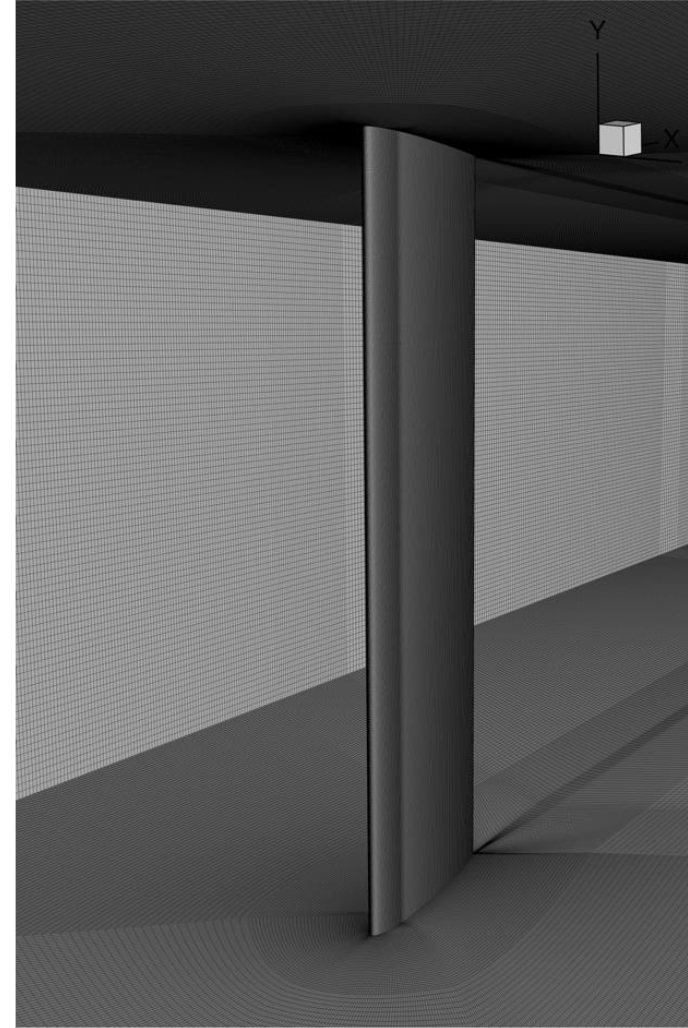
\includegraphics[
                height=0.56\textheight,
                width=\textwidth,
                keepaspectratio,
                trim={0cm 0cm 0cm 0cm},
                clip
            ]{FIGURES_CONDITIONS/NACA0012_MESH_VIEW.png}

            \vspace{0.05cm}

            {\scriptsize\textbf{Mesh Tunnel View}}
        \end{column}

        \hfill

        % ----------------------------------------------------
        % Integration patch
        % ----------------------------------------------------
        \begin{column}{0.49\textwidth}
            \centering

            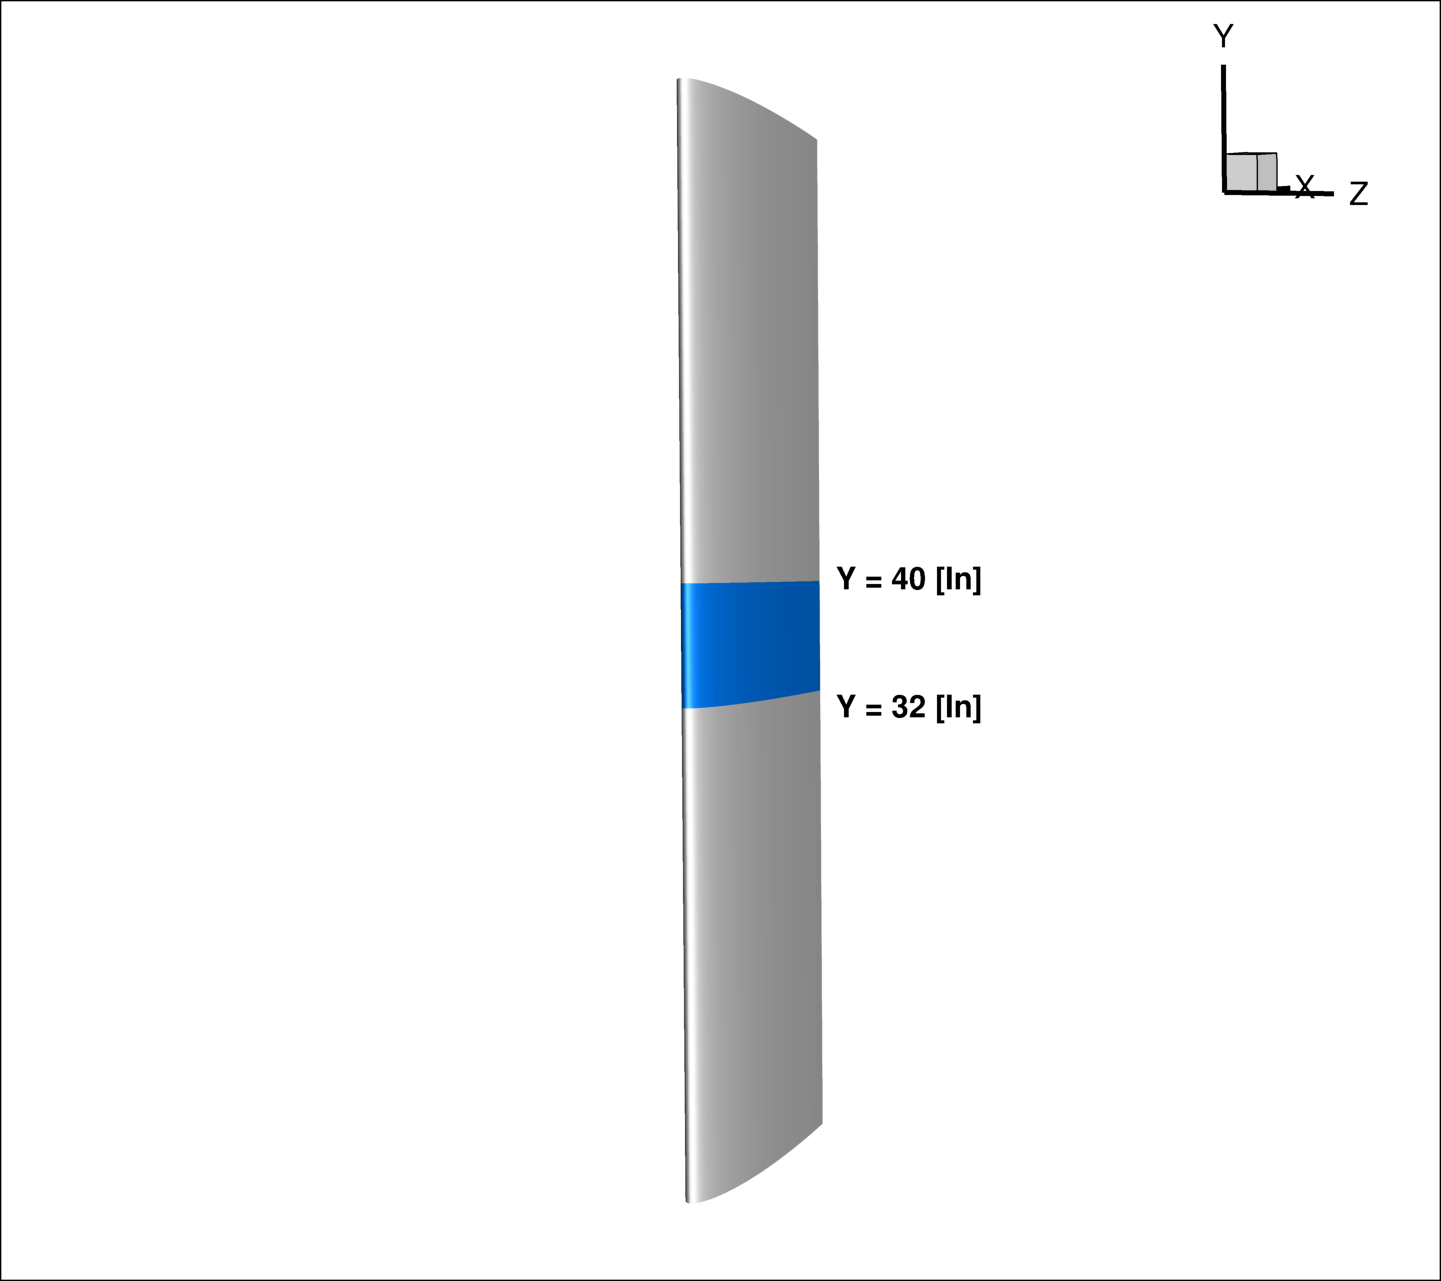
\includegraphics[
                width=\textwidth,
                trim={10cm 0.1cm 10cm .1cm},
                clip
            ]{FIGURES_CONDITIONS/NACA0012_INTEGRATION_PATCH.png}

            \vspace{-0.2cm}

            {\scriptsize\textbf{Integration Patch}}
        \end{column}

    \end{columns}
\end{figure}

\vspace{-0.25cm}

\centering
\begin{tabular}{lcc}
\toprule
\textbf{Grid} & \textbf{Nodes} & \textbf{Elements} \\
\midrule
L1 & $60.45$ M & $59.86$ M \\
L2 & $27.31$ M & $26.99$ M \\
L3 & $11.23$ M & $11.08$ M \\
L4 & $5.95$ M  & $5.86$ M \\
\bottomrule
\end{tabular}

\end{column}

%------------------------------------------------
\begin{column}{0.53\textwidth}
\centering

\textbf{Icing Conditions} \\
\vspace{0.05cm}

\begin{tabular}{lcc}
\toprule
 & \textbf{AE3932} & \textbf{AE3933} \\
\midrule
$T_{0,\mathrm{ref}}$ [K]         & $267.51$ & $271.0$ \\
$T_{s,\mathrm{ref}}$ [K]         & $262.305$ & $265.8$ \\
$M_{\mathrm{ref}}$ [-]           & $0.3151$ & $0.3127$ \\
$U_{\mathrm{ref}}$ [m/s]         & $102.31$ & $102.19$ \\
$\rho_{\mathrm{ref}}$ [kg/m$^3$] & $1.21$ & $1.2$ \\
$Re_{c,\mathrm{ref}}$ [-]        & $3.9795\times10^6$ & $3.8947\times10^6$ \\
LWC [g/m$^3$]                     & $0.55$ & $0.55$ \\
MVD [$\mu$m]                      & $20$ & $20$ \\
Exposure time [min]               & $7$ & $7$ \\
\midrule
\textbf{Exp. ice mass [g]}        & \textbf{101.0} & \textbf{85.9} \\
\bottomrule
\end{tabular}


\vspace{-0.1cm}

\begin{block}{\scriptsize Analysis Setup}
\scriptsize

\begin{itemize}
    \item \textbf{Data Extraction:}
    Aerodynamic coefficients integrated over the full profile span ($Y=0$--$72$ in);
    icing quantities over the highlighted patch ($Y=32$--$40$ in); slices extracted at
    $Y=36$ in.

    \item \textbf{Droplet Distribution:}
    1-, 3-, 7-, and 15-bin distributions with preserved total LWC
    across all grid levels.
\end{itemize}

\end{block}

\end{column}
\end{columns}
\end{frame}

% ============================================================
% Participants
% ============================================================

\begin{frame}{\small IPW3 -- NACA0012 Case Participants}
\scriptsize

\definecolor{p001}{HTML}{2CA02C}
\definecolor{p002}{HTML}{17BECF}
\definecolor{p003}{HTML}{00695C}
\definecolor{p004}{HTML}{BCBD22}
\definecolor{p006}{HTML}{9467BD}
\definecolor{p007}{HTML}{1F77B4}
\definecolor{p008}{HTML}{D62728}
\definecolor{p009}{HTML}{A5006A}
\definecolor{p010}{HTML}{0047FF}
\definecolor{p013}{HTML}{637939}
\definecolor{p014}{HTML}{E377C2}
\definecolor{p015}{HTML}{393B79}
\definecolor{p019}{HTML}{E6550D}
\definecolor{p020}{HTML}{843C39}

\centering

\renewcommand{\arraystretch}{1.20}
\setlength{\tabcolsep}{8pt}

\begin{tabular}{ccc}
\toprule
\textbf{ID} &
\textbf{Participant / Organization} &
\textbf{Line Color} \\
\midrule

001 & CIRA                   & \textcolor{p001}{\rule{1.5cm}{1.5pt}} \\
002 & AeroTex                & \textcolor{p002}{\rule{1.5cm}{1.5pt}} \\
003 & NRC                    & \textcolor{p003}{\rule{1.5cm}{1.5pt}} \\
004 & ONERA                  & \textcolor{p004}{\rule{1.5cm}{1.5pt}} \\
006 & Dassault               & \textcolor{p006}{\rule{1.5cm}{1.5pt}} \\
007 & Polytechnique Montréal & \textcolor{p007}{\rule{1.5cm}{1.5pt}} \\
008 & Collins Aerospace      & \textcolor{p008}{\rule{1.5cm}{1.5pt}} \\
009 & Sikorsky               & \textcolor{p009}{\rule{1.5cm}{1.5pt}} \\
010 & NASA                   & \textcolor{p010}{\rule{1.5cm}{1.5pt}} \\
013 & Boeing                 & \textcolor{p013}{\rule{1.5cm}{1.5pt}} \\
014 & Airbus                 & \textcolor{p014}{\rule{1.5cm}{1.5pt}} \\
019 & Synopsys               & \textcolor{p019}{\rule{1.5cm}{1.5pt}} \\
020 & Bombardier             & \textcolor{p020}{\rule{1.5cm}{1.5pt}} \\

\bottomrule
\end{tabular}

\end{frame}

% ============================================================
%  Data Received
% ============================================================

\begin{frame}{\small  Summary of Submitted Data}
\tiny

\centering

\begin{columns}[T,onlytextwidth]

% ============================================================
% AE3932
% ============================================================
\begin{column}{0.495\textwidth}
\centering

\textbf{AE3932}

\vspace{0.05cm}

\renewcommand{\arraystretch}{1.10}
\setlength{\tabcolsep}{1.05pt}

\begin{tabular}{c|cccc|cccc|cccc|cccc}
\toprule
&
\multicolumn{4}{c|}{\textbf{L1}} &
\multicolumn{4}{c|}{\textbf{L2}} &
\multicolumn{4}{c|}{\textbf{L3}} &
\multicolumn{4}{c}{\textbf{L4}} \\

\textbf{ID}
& 1 & 3 & 7 & 15
& 1 & 3 & 7 & 15
& 1 & 3 & 7 & 15
& 1 & 3 & 7 & 15 \\
\midrule

001 & \checkmark&&& & \checkmark&&& & \checkmark&&& & \checkmark&&& \\
002 & &\checkmark&\checkmark&\checkmark & &\checkmark&\checkmark&\checkmark & &\checkmark&\checkmark&\checkmark & &\checkmark&\checkmark&\checkmark \\
003 & &&& & \checkmark&\checkmark&\checkmark&\checkmark & \checkmark&\checkmark&\checkmark&\checkmark & \checkmark&\checkmark&\checkmark&\checkmark \\
004 & \checkmark&\checkmark&\checkmark&\checkmark & \checkmark&\checkmark&\checkmark&\checkmark & \checkmark&\checkmark&\checkmark&\checkmark & \checkmark&\checkmark&\checkmark&\checkmark \\
006 & &&&\checkmark & &&&\checkmark & &&& & &&&\checkmark \\
007 & \checkmark&\checkmark&\checkmark&\checkmark & \checkmark&\checkmark&\checkmark&\checkmark & \checkmark&\checkmark&\checkmark&\checkmark & \checkmark&\checkmark&\checkmark&\checkmark \\
008 & \multicolumn{4}{c|}{} & \multicolumn{4}{c|}{} & \multicolumn{4}{c|}{} & \multicolumn{4}{c}{} \\
009 & \multicolumn{4}{c|}{} & \multicolumn{4}{c|}{} & \multicolumn{4}{c|}{} & \multicolumn{4}{c}{} \\
010 & \checkmark&\checkmark&\checkmark&\checkmark & \checkmark&\checkmark&\checkmark&\checkmark & \checkmark&\checkmark&\checkmark&\checkmark & \checkmark&\checkmark&\checkmark&\checkmark \\
013 & &&&\checkmark & &&&\checkmark & &&& & &&& \\
014 & \checkmark&\checkmark&\checkmark&\checkmark & \checkmark&\checkmark&\checkmark&\checkmark & \checkmark&\checkmark&\checkmark&\checkmark & \checkmark&\checkmark&\checkmark&\checkmark \\
015 & &&& & &&& & &&& & &&& \\
019 & \checkmark&\checkmark&\checkmark&\checkmark & \checkmark&\checkmark&\checkmark&\checkmark & \checkmark&\checkmark&\checkmark&\checkmark & \checkmark&\checkmark&\checkmark&\checkmark \\
020 & &&&\checkmark & &&&\checkmark & \checkmark&\checkmark&\checkmark&\checkmark & &&&\checkmark \\

\midrule
\textbf{Total}
& \textbf{6} & \textbf{6} & \textbf{6} & \textbf{9}
& \textbf{7} & \textbf{7} & \textbf{7} & \textbf{10}
& \textbf{8} & \textbf{8} & \textbf{8} & \textbf{8}
& \textbf{7} & \textbf{7} & \textbf{7} & \textbf{9} \\
\bottomrule
\bottomrule
\end{tabular}

\end{column}


% ============================================================
% AE3933
% ============================================================
\begin{column}{0.495\textwidth}
\centering

\textbf{AE3933}

\vspace{0.05cm}

\renewcommand{\arraystretch}{1.10}
\setlength{\tabcolsep}{1.05pt}

\begin{tabular}{c|cccc|cccc|cccc|cccc}
\toprule
&
\multicolumn{4}{c|}{\textbf{L1}} &
\multicolumn{4}{c|}{\textbf{L2}} &
\multicolumn{4}{c|}{\textbf{L3}} &
\multicolumn{4}{c}{\textbf{L4}} \\

\textbf{ID}
& 1 & 3 & 7 & 15
& 1 & 3 & 7 & 15
& 1 & 3 & 7 & 15
& 1 & 3 & 7 & 15 \\
\midrule

001 & \checkmark&\checkmark&\checkmark&\checkmark & \checkmark&&& & \checkmark&&& & \checkmark&&& \\
002 & &\checkmark&\checkmark&\checkmark & &\checkmark&\checkmark&\checkmark & &\checkmark&\checkmark&\checkmark & &\checkmark&\checkmark&\checkmark \\
003 & &&& & \checkmark&\checkmark&\checkmark&\checkmark & \checkmark&\checkmark&\checkmark&\checkmark & \checkmark&\checkmark&\checkmark&\checkmark \\
004 & \checkmark&\checkmark&\checkmark&\checkmark & \checkmark&\checkmark&\checkmark&\checkmark & \checkmark&\checkmark&\checkmark&\checkmark & \checkmark&\checkmark&\checkmark&\checkmark \\
006 & &&&\checkmark & &&&\checkmark & &&& & &&& \\
007 & \checkmark&\checkmark&\checkmark&\checkmark & \checkmark&\checkmark&\checkmark&\checkmark & \checkmark&\checkmark&\checkmark&\checkmark & \checkmark&\checkmark&\checkmark&\checkmark \\
008 & \checkmark&\checkmark&\checkmark&\checkmark & \checkmark&\checkmark&\checkmark&\checkmark & \checkmark&\checkmark&\checkmark&\checkmark & \checkmark&\checkmark&\checkmark&\\
009 & \checkmark&&& & \checkmark&&& & \checkmark&&& & \checkmark&&& \\
010 & \checkmark&\checkmark&\checkmark&\checkmark & \checkmark&\checkmark&\checkmark&\checkmark & \checkmark&\checkmark&\checkmark&\checkmark & \checkmark&\checkmark&\checkmark&\checkmark \\
013 & &&&\checkmark & &&&\checkmark & &&& & &&& \\
014 & \checkmark&\checkmark&\checkmark&\checkmark & \checkmark&\checkmark&\checkmark&\checkmark & \checkmark&\checkmark&\checkmark&\checkmark & \checkmark&\checkmark&\checkmark&\checkmark \\
015 & &&& & &&& & &&& & &&& \\
019 & \checkmark&\checkmark&\checkmark&\checkmark & \checkmark&\checkmark&\checkmark&\checkmark & \checkmark&\checkmark&\checkmark&\checkmark & \checkmark&\checkmark&\checkmark&\checkmark \\
020 & &&& & &&& & &&&\checkmark & &&& \\

\midrule
\textbf{Total}
& \textbf{8} & \textbf{8} & \textbf{8} & \textbf{10}
& \textbf{9} & \textbf{8} & \textbf{8} & \textbf{10}
& \textbf{9} & \textbf{8} & \textbf{8} & \textbf{9}
& \textbf{9} & \textbf{8} & \textbf{8} & \textbf{7} \\
\bottomrule
\bottomrule
\end{tabular}
\end{column}
\end{columns}

% \vspace{0.2cm}

% \parbox{0.98\textwidth}{\scriptsize\raggedright
% \centering
% \checkmark: populated CutData received for the corresponding droplet-bin distribution. 
% }

\end{frame}


% ============================================================
% Modeling Choices
% ============================================================

\begin{frame}{\small Modeling Choices Across Submissions}
\scriptsize

\centering

% ------------------------------------------------------------
% Modeling choices table
% ------------------------------------------------------------

{\tiny
\renewcommand{\arraystretch}{1.45}
\setlength{\tabcolsep}{1.65pt}

\begin{tabular}{c|ccccccccccc}
\toprule
\textbf{Model / Method}
& \textbf{001}
& \textbf{002}
& \textbf{003}
& \textbf{004}
& \textbf{007}
& \textbf{008}
& \textbf{009}
& \textbf{010}
& \textbf{013}
& \textbf{014}
& \textbf{019} \\
\midrule

\textbf{Turbulence}
& $k$--$\omega$ TNT
& $k$--$\omega$ SST
& SST-QCR
& $k$--$\omega$ SST
& SA
& $k$--$\omega$ SST
& $k$--$\omega$ SST
& SA-neg-QCR
& SA
& SA-neg
& $k$--$\omega$ SST \\

\textbf{Droplet formulation}
& Eul.
& Lag.
& Lag.
& Eul.
& Eul.
& Eul.
& Eul.
& Lag.
& Lag.
& Lag.
& Eul. \\

\textbf{HTC method}
& --
& BL Int.
& 1-sol. + $T_{rec}$
& 1-sol. + $T_{rec}$
& $T_{rec}$
& EID
& $T_{rec}$
& 2 $T_w$
& 1-sol. + RA
& BL Int. + RA
& -- \\

\textbf{Thermodynamics}
& Mess.
& Mess.
& Mess.
& Mess.
& Mess.
& ICE3D/EID
& SWIM
& Mess.
& Mess.
& Mess.
& SWIM+ \\

\textbf{Geometry evolution}
& Lag./IB
& Interp.
& Pseudo-trans.
& Alg.
& Lag.
& ALE
& --
& Prism. extr.
& Extr.
& Alg.
& Lag./remesh \\

\bottomrule
\end{tabular}
}

\vspace{0.10cm}

% ------------------------------------------------------------
% Abbreviations
% ------------------------------------------------------------

\begin{minipage}{0.98\textwidth}
\tiny
\textit{
Eul. = Eulerian;
Lag. = Lagrangian;
SA = Spalart--Allmaras;
SA-neg = negative SA;
QCR = quadratic constitutive relation;
BL Int. = boundary-layer integral;
$T_{rec}$ = recovery temperature;
$T_w$ = wall temperature;
1-sol. = one-solution method;
RA = Reynolds analogy;
EID = extended icing data;
Mess. = Messinger;
SWIM = shallow-water icing model;
IB = immersed boundary;
ALE = arbitrary Lagrangian--Eulerian;
Alg. = algebraic;
Interp. = interpolation;
Extr. = extrusion;
Prism. extr. = prismatoid extrusion;
Pseudo-trans. = pseudo-transient;
-- = not reported.
}
\end{minipage}

% ------------------------------------------------------------
% Overall trends
% ------------------------------------------------------------
\vspace{-0.05cm}

\begin{block}{\scriptsize Overall Trends}
\begin{itemize}

    \item \textbf{Turbulence:}
    $k$--$\omega$-family formulations predominate (\textbf{64\%}),
    with \textbf{36\%} using SA-family formulations.

    \item \textbf{Droplets:}
    Eulerian formulations are slightly predominant (\textbf{55\%}),
    with \textbf{45\%} Lagrangian.

    \item \textbf{Heat transfer:}
    A variety of approaches are used, including recovery-temperature,
    boundary-layer integral/Reynolds-analogy, two-$T_w$, one-solution,
    and other methods.

    \item \textbf{Thermodynamics:}
    Messinger-based approaches predominate (\textbf{73\%}), with
    SWIM-based methods also represented.

    \item \textbf{Geometry evolution:}
    Diverse approaches are used, including algebraic,
    displacement/extrusion, ALE, interpolation, remeshing,
    and pseudo-transient methods.

    \item \textbf{Notable approaches:}
    One submission employs an immersed-boundary formulation, while
    another uses a morphogenetic approach.

    \item \textbf{Ice accretion:}
    Workshop comparisons focus on single-shot results;
    2 participants also submitted multilayer/multishot results.

\end{itemize}
\end{block}

\vspace{-0.25cm}
\begin{flushleft}
{\tiny\textcolor{red}{*} Based on reported data only.}
\end{flushleft}

\end{frame}